% ============================================================
%  MTP Phase 2 Report
%  Title: Anonymity Preserving in Lightweight and Decoupled
%         Distributed Authentication for Multihop IoT Networks
%  Author: Anup Kulkarni, Roll No: 244101005
%  Guide:  Dr. Manas Khatua
%  Dept:   CSE, IIT Guwahati
% ============================================================

\documentclass[12pt,a4paper]{report}

% ---- Page geometry ----
\usepackage[top=1in,bottom=1in,left=1.25in,right=1in]{geometry}

% ---- Core packages ----
\usepackage{graphicx}
\usepackage{amsmath,amssymb,amsfonts}
\usepackage{booktabs}
\usepackage{multirow}
\usepackage{array}
\usepackage{tabularx}
\usepackage{float}
\usepackage{caption}
\usepackage{subcaption}
\usepackage{placeins}
\usepackage{setspace}
\setlength{\parskip}{6pt}
\setlength{\parindent}{0pt}
\usepackage{tikz}
\usetikzlibrary{arrows.meta,positioning,shapes.geometric}
\usepackage{algorithm}
\usepackage{algpseudocode}
\usepackage{url}
\usepackage{cite}

% ---- Hyperlinks (load last among setup packages) ----
\usepackage[colorlinks=true,linkcolor=black,citecolor=blue,urlcolor=blue]{hyperref}

% ---- Figure path: look in current dir, then Paper/ ----
\graphicspath{{./}{../Paper/}{../Diagrams/diagrams/}}

% ---- Line spacing ----
\onehalfspacing

% ---- Chapter heading style ----
\usepackage{titlesec}
\titleformat{\chapter}[display]
  {\normalfont\Large\bfseries\centering}
  {\chaptertitlename\ \thechapter}{12pt}{\LARGE}
\titlespacing*{\chapter}{0pt}{-20pt}{30pt}

% ============================================================
\begin{document}

% ============================================================
%  TITLE PAGE
% ============================================================
\begin{titlepage}
  \centering
  \vspace*{0.8cm}

  {\LARGE\bfseries Anonymity Preserving in Lightweight and\\[5pt]
   Decoupled Distributed Authentication for\\[5pt]
   Multihop IoT Networks\par}

  \vspace{0.35cm}
  {\large\itshape MTP Phase 2 Report\par}

  \vfill

  {\normalsize Master of Technology\par}
  {\normalsize \textit{in}\par}
  {\normalsize\bfseries Computer Science \& Engineering\par}

  \vspace{0.55cm}
  {\normalsize \textit{by}\par}
  \vspace{0.15cm}
  {\large\bfseries Anup Kulkarni\par}
  {\normalsize Roll No.: 244101005\par}

  \vspace{0.55cm}
  {\normalsize\itshape Under the Guidance of\par}
  \vspace{0.15cm}
  {\large\bfseries Dr.\ Manas Khatua\par}

  \vfill

  
\includegraphics[width=0.23\textwidth]{IITG_logo}

  \vspace{0.5cm}
  {\normalsize Department of Computer Science \& Engineering\par}
  {\large Indian Institute of Technology Guwahati\par}
  {\normalsize Guwahati -- 781039, India\par}
  \vspace{0.35cm}
  {\normalsize 2025--2026\par}
  \vspace*{0.6cm}
\end{titlepage}

% ============================================================
%  FRONT MATTER  (roman numerals)
% ============================================================
\pagenumbering{roman}

% ---- Abstract ----
\chapter*{Abstract}
\addcontentsline{toc}{chapter}{Abstract}
\setcounter{page}{1}

The primary objective of this work is to identify, address, and validate critical
security and privacy gaps in the lightweight decoupled distributed authentication
scheme for multihop IoT networks proposed in~\cite{das2026comsnets}.
Two significant vulnerabilities were identified.
First, the real device identity $ID_D$ is transmitted in plaintext over the public
channel during every authentication session.
This exposure enables any passive adversary to track devices across sessions,
correlate repeated authentication attempts, and infer network behaviour, constituting
a direct violation of modern privacy requirements.
Second, when a key-exchange packet is lost in transit, the device and authentication
server hold divergent session states, causing all subsequent authentication attempts
to fail and forcing the device through a costly full re-enrolment.

To address both vulnerabilities, this work proposes an anonymity-preserving and
desynchronisation-resilient extension of the base scheme.
Per-session pseudonym rotation replaces the real identity $ID_D$ in all
open-channel communications with a rotating pseudonym
$\mathit{PID} = H(ID_D \| m_{\mathrm{curr}})$, refreshed after each successful
key exchange, so that successive pseudonyms are computationally unlinkable.
A dual-state mechanism maintained at the authentication server stores both the
current and the immediately preceding session state, enabling seamless recovery
from a single packet-loss event without re-enrolment.
All 19 ProVerif queries are satisfied under the Dolev--Yao adversary model,
confirming authentication correspondence, session key secrecy, forward secrecy,
anonymity preservation, and offline guessing resistance.
COOJA/Contiki-NG simulations on a 100-node RPL network show a 42.8\,\% reduction
in per-device energy over LAAKA~\cite{ali2024laaka} and 34.6\,\% over
Zhou~\cite{zhou2024auth}, while hardware measurements on Raspberry Pi~4B confirm
52.5\,\% and 14.2\,\% reductions respectively.

\clearpage

% ---- Table of Contents ----
\tableofcontents
\clearpage

% ---- List of Tables ----
\listoftables
\clearpage

% ---- List of Figures ----
\listoffigures
\clearpage

% ============================================================
%  MAIN MATTER  (arabic numerals)
% ============================================================
\pagenumbering{arabic}

% ============================================================
%  CHAPTER 1 — Introduction
% ============================================================
\chapter{Introduction}

The Internet of Things (IoT) has grown very fast in the last few years and has become
the main technology behind many smart systems like factories, smart grids, health
monitoring, and transport networks.
These systems use a large number of small and low-power devices that communicate over
wireless links that are open to everyone.
Because of this, having a secure and quick authentication method is important to
protect IoT setups from attacks like impersonation, replay, man-in-the-middle, key
leaks, or even device capture.

A large number of lightweight authentication methods have been proposed to deal with
the low processing power and limited energy of IoT devices.
Many works use Physical Unclonable Functions (PUFs), simple hash-based
challenge--response mechanisms, and symmetric key constructions, because these do
not cost much to compute.
The base protocol used in this work follows the same direction: it uses PUFs, avoids
long-term key storage, works in a decoupled way across nodes, and supports multihop
verification with very low cost~\cite{das2026comsnets}.

But even with all this, there is still a privacy problem.
During authentication, the device's real identity $ID_D$ is sent openly on the
public channel.
This leaks the identity and makes it easy for attackers to track the device, link
different sessions, or even plan targeted attacks on that specific device.

Recent research shows that identity privacy in IoT authentication is not just an extra
feature but a basic requirement.
Many surveys on lightweight anonymous authentication point out that anonymity,
untraceability, and forward secrecy are important, especially when devices operate
in open environments~\cite{zhong2025survey}.
There are already some anonymity ideas like changing pseudonym IDs every session or
using hash-chain-based temporary identities, but these often bring new issues like
desynchronisation, large storage, slow identity lookup, or high computation.
Frameworks like SF3-UA, SF5-UA, SF6-UA, and forward secrecy methods like SF7-FS,
SF8-FS, and SF9-FS show how difficult it is to design a scheme that gives anonymity,
unlinkability, and still stays safe when messages are lost~\cite{zhong2025survey}.

Because of these points, this work focuses on how anonymity features can be added to
the chosen PUF-based scheme without breaking its lightweight nature.
In the current protocol, all authentication messages go through a public channel, so
sending the real device identity $ID_D$ makes it possible for attackers to follow the
device, relate old and new sessions, or even impersonate it.
To solve this, this work studies anonymous authentication methods from earlier works
and finds a simple and low-cost method that fits into the base scheme.
The goal is to achieve identity anonymity, unlinkability, and non-traceability while
still keeping the protocol light enough for IoT devices.

A second gap identified in the base scheme is its lack of desynchronisation
resilience.
Because the base scheme stores only one session nonce at the authentication server,
any packet loss during the key exchange phase causes the device and server states to
diverge, leading to a permanent denial-of-service condition that requires costly
full re-enrolment to repair.

This work makes the following key contributions:
\begin{enumerate}
  \item An improved scheme over Das~\cite{das2026comsnets} is proposed, adding
    per-session pseudonym rotation for device anonymity and a dual-state
    desynchronisation recovery mechanism.
  \item The security of the proposed scheme is validated through both informal
    analysis and formal verification using ProVerif under the Dolev--Yao adversary
    model.
  \item The efficiency of the proposed scheme is evaluated using theoretical analysis,
    COOJA/Contiki-NG simulation-based framework, and hardware implementation on
    Raspberry Pi~4B, emphasising communication overhead, energy consumption, and CPU
    utilisation in a multihop constrained setting.
\end{enumerate}

The rest of this report is organised as follows.
Chapter~2 surveys the related literature.
Chapter~3 describes the prerequisite concepts.
Chapter~4 overviews the base authentication scheme.
Chapter~5 presents the proposed scheme in full detail.
Chapter~6 contains the security analysis.
Chapter~7 presents the performance evaluation.
Chapter~8 discusses future scope.
Chapter~9 concludes the report.

% ============================================================
%  CHAPTER 2 — Literature Survey
% ============================================================
\chapter{Literature Survey}

Recent work in IoT authentication has moved more towards lightweight and distributed
methods, mainly because old centralised systems put too much load on one gateway and
also create a single point of failure.
Since IoT devices have very low power and limited memory, researchers started looking
for ways where many nodes can share the authentication work.

\textbf{Light-SAE}~\cite{rosa2023lightsae} is one example of this shift.
It lets already authenticated nodes help new ones join using a simple challenge and
response idea.
It uses TinyJAMBU for lightweight encryption and a modified Diffie--Hellman step to
set the session key in multihop networks.
This reduces the load on the gateway.
But the problem is that Light-SAE still sends the node identity in plain form and
gives no protection for anonymity or unlinkability.
So it is not very safe for places where privacy is important.

Another scheme, \textbf{SAKMS}~\cite{yang2024sakms}, is made for industrial IoT
systems that follow the 6TiSCH setup.
It uses ECC to do mutual authentication and also uses ECQV certificates.
It also improves key management and gives strong forward secrecy.
The scheme was checked using ProVerif.
But because SAKMS uses many elliptic-curve operations, it becomes heavy for very
small IoT devices.
Also, SAKMS still uses fixed device IDs inside the messages, so the devices can be
tracked easily.
These issues show that strong security does not always mean privacy and lightweight
performance.

The \textbf{base decoupled PUF-based authentication scheme}~\cite{das2026comsnets}
solves many of these problems by using PUFs to avoid storing long-term secrets and
by using a hash-based accumulator to check membership.
It is decoupled, meaning both parent and non-parent nodes can work as authentication
servers, which helps spread the load in multihop networks.
It only uses simple things like hash, XOR, and two AES calls, so it is very light
to run.
But its main weakness is that it sends the device identity ($ID_D$) directly during
authentication.
Because all the messages travel over a public channel, an attacker can easily read
the identity, follow the device over time, or even plan targeted attacks.
So keeping identity private is important.

To solve such privacy issues, many anonymous authentication schemes have been
proposed.
\textbf{He~et~al.}~\cite{he2023lightweight} achieve lightweight anonymous
authentication using hash-and-XOR primitives for CoAP/OSCORE but rely on a
centralised server, removing the decoupled-distribution advantage.
\textbf{LAAKA}~\cite{ali2024laaka} is another lightweight anonymous scheme that uses
ECC to protect the identity while doing mutual authentication.
But again, ECC operations cost more power and may not fit very small IoT nodes.

There is also a comprehensive survey on lightweight anonymous
authentication~\cite{zhong2025survey} that lists methods like temporary pseudonyms,
PUF-assisted anonymous login, hidden membership proofs using accumulators, and
unlinkable tokens.
The survey also explains common problems like desynchronisation, pseudonym
exhaustion, and replay protection, which must be considered when adding anonymity to
IoT systems.
Their taxonomy deconstructs existing protocols into nine sub-frameworks (SF1-UA
through SF9-FS) and two general frameworks (GF1, GF2), and their analysis
demonstrates that only GF2 simultaneously achieves user anonymity, forward secrecy,
and desynchronisation resistance.

\textbf{Zhou~et~al.}~\cite{zhou2024auth} propose a security-enhanced lightweight
and anonymity-preserving user authentication scheme for IoT-based healthcare,
providing hash-based anonymous authentication with nonce masking to protect sensitive
metadata over open wireless channels.

Other works use \textbf{blockchain}~\cite{ahmed2023chains} and
\textbf{certificateless cryptography}~\cite{alriyami2003cert} to achieve
decentralisation and identity hiding, but they incur prohibitive storage and consensus
overhead.
\textbf{Li~et~al.}~\cite{li2020puf} and \textbf{Zheng~et~al.}~\cite{zheng2022puf}
combine PUF with session key exchange but do so at the cost of ECC operations that
are too heavy for highly constrained nodes.

Even with all these works, there is still a clear gap.
None of the schemes combine all these things together: (i)~decoupled authentication,
(ii)~PUF-based secrecy without long-term keys, (iii)~very low computation, and
(iv)~anonymity with unlinkability and desynchronisation recovery.
This is why this work focuses on building an anonymous version of the base PUF-based
protocol so that no device identity is revealed on the public channel, while still
keeping the scheme lightweight and distributed.

To show the differences between all these methods clearly, Table~\ref{tab:features}
lists the use of decoupling, PUF, accumulator-based authentication, authentication
secret update, anonymity, desynchronisation recovery, and the computation and
communication overhead for all the schemes studied.

\begin{table}[H]
  \centering
  \caption{Features Comparison of Authentication Schemes.}
  \label{tab:features}
  \small
  \setlength{\tabcolsep}{5pt}
  \begin{tabular}{lcccccccc}
    \toprule
    Scheme & Dec. & PUF & Acc. & ASU & Anon. & Desync & C.OH & M.OH \\
    \midrule
    RAAF-MEC~\cite{alruwaili2025raaf}   & $\times$ & \checkmark & $\times$ & \checkmark & $\times$ & $\times$ & H & L \\
    SAKMS~\cite{yang2024sakms}          & \checkmark & $\times$ & $\times$ & $\times$ & $\times$ & $\times$ & H & L \\
    Li et al.~\cite{li2020puf}          & \checkmark & \checkmark & $\times$ & \checkmark & $\times$ & $\times$ & H & L \\
    Zheng et al.~\cite{zheng2022puf}    & \checkmark & \checkmark & $\times$ & \checkmark & $\times$ & $\times$ & M & L \\
    Das et al.~\cite{das2026comsnets}   & \checkmark & \checkmark & \checkmark & \checkmark & $\times$ & $\times$ & L & L \\
    \textbf{Proposed}                  & \checkmark & \checkmark & \checkmark & \checkmark & \checkmark & \checkmark & \textbf{L} & \textbf{L} \\
    \bottomrule
  \end{tabular}\\[5pt]
  \raggedright\small
  \textit{Dec.}: Decoupled design.\quad
  \textit{Acc.}: Hash-based accumulator.\quad
  \textit{ASU}: Auth.\ secret update.\\
  \textit{Anon.}: Device anonymity via pseudonym.\quad
  \textit{Desync}: Desync.\ recovery.\\
  \textit{C.OH}: Computation — L (Hash/XOR/$\le$2 AES), M ($>$2 AES), H (ECC/Pairings).\\
  \textit{M.OH}: Message exchanges — L (1--3), M (4--5), H ($>$5).
\end{table}

% ============================================================
%  CHAPTER 3 — Prerequisites for Objective
% ============================================================
\chapter{Prerequisites for Objective}

\section{Physically Unclonable Function}

A Physically Unclonable Function (PUF) constitutes a one-way physical function that
generates a unique response $R$ for a challenge $C$ selected from a pool of
challenge space $\mathcal{C}$.
PUFs exploit uncontrollable manufacturing variations inherent in integrated circuits,
which are practically impossible to replicate.
Various types of PUFs have been proposed, including SRAM PUFs, Arbiter PUFs, and
Ring Oscillator (RO) PUFs.
In this work, a Ring Oscillator PUF is used due to its higher execution speed and
lower overhead.

A function is considered a valid and secure PUF if it satisfies the following
properties:

\begin{itemize}
  \item \textbf{Evaluatable:} A legitimate entity can easily compute a response
    $R \in \mathcal{R}$ for any given challenge $C \in \mathcal{C}$.

  \item \textbf{Unpredictability:} An adversary cannot predict the response $R$ for
    any challenge $C$ without physical access to the PUF.

  \item \textbf{Uniqueness:} For two different PUF instances, $\mathsf{PUF}_1$ and
    $\mathsf{PUF}_2$, the probability that
    $\mathsf{PUF}_1(C) = \mathsf{PUF}_2(C)$ for the same challenge $C$ is
    negligible.

  \item \textbf{Reliability:} For a fixed challenge $C$, the PUF response
    $\mathsf{PUF}(C) = R$ remains stable over time and environmental variations.

  \item \textbf{One-wayness:} Given a response $R$, it is computationally infeasible
    to determine the corresponding challenge $C$ or invert the PUF.
\end{itemize}

These properties enable PUFs to serve as intrinsic, hardware-bound secrets for secure
key generation, device binding, and authentication in resource-constrained IoT
systems.

\section{Hash-based One-Way Accumulator}

A one-way hash accumulator, proposed as an efficient alternative to digital
signatures in authentication protocols, provides a compact, non-invertible
representation of a set of elements.
In such an accumulator, multiple items can be combined using a quasi-commutative
operator such that the final accumulated value is independent of the order in which
elements are processed.

Formally, a function
\[
  f : A \times B \to A
\]
is said to be quasi-commutative if, for all $a \in A$ and for all $b, c \in B$,
\begin{equation}
  f(f(a,b),c) = f(f(a,c),b).
\end{equation}

Nyberg introduced a fast accumulated hashing method suitable for lightweight systems.
Let $N$ denote the maximum number of accumulable items, and let
$h : \{0,1\}^* \to \{0,1\}^\ell$ be a cryptographically secure hash function.
Given a set of items $Y = \{y_1, y_2, \ldots, y_m\}$, $m \le N$, each item is
first hashed as $Y_i = h(y_i)$, $i = 1, 2, \ldots, m$.
The accumulated hash is then computed as:
\begin{equation}
  T_{\mathsf{Acc}} = H(s, Y) = s \bigodot_{i=1}^{m} h(y_i),
\end{equation}
where $s$ is an initialisation seed and $\bigodot$ represents the bitwise AND
operator.
Since the AND operator is commutative and the hash function is one-way, the
accumulator inherits quasi-commutative and one-way properties.

\textbf{Membership Verification:} To verify whether an item $y_i$ belongs to the
accumulated set, compute $Y_i = h(y_i)$, and check whether
$Y_i \bigodot T_{\mathsf{Acc}} = T_{\mathsf{Acc}}$.

The security of the accumulator depends on the difficulty of forging a value $Y_i$
that passes verification.
For a security parameter $t$, the required length $r$ of the accumulated hash is
given by $r = N \times e \times t$, where $e$ is Euler's (Napier's) constant.

\section{Core Concept of Anonymity Preserving}

In IoT security, anonymity is defined by two key properties:
\textbf{Untraceability} (concealing the sender's real identity) and
\textbf{Unlinkability} (preventing the correlation of multiple sessions to a single
device).
While simply encrypting a static ID protects the credential itself, it does not
prevent traffic analysis; if the encrypted value remains constant, an adversary can
track the device's activity patterns.

To achieve robust anonymity, modern schemes utilise \textbf{Dynamic Pseudonyms}.
Instead of a static identifier, the device generates a session-specific alias
($\mathit{PID}$) using a shared secret or random nonce, e.g.,
$\mathit{PID}_{i+1} = H(\mathit{ID} \| \mathit{Nonce}_i)$.
To an external observer, each authentication request appears as a fresh, random
string of bits, completely uncorrelated with previous sessions.

A critical challenge when using dynamic pseudonyms is \textbf{desynchronisation}.
If the message carrying the new nonce is lost in transit, the device retains the old
nonce while the server has already advanced to the new one.
Their pseudonym computations then diverge, and all subsequent authentications fail.
To handle this gracefully, a dual-state storage approach retains both the current and
the immediately previous state at the server, allowing recovery without re-enrolment.

% ============================================================
%  CHAPTER 4 — Base Scheme
% ============================================================
\chapter{Base Scheme}

\section{Overview of the Base Authentication Scheme}

The base scheme~\cite{das2026comsnets} is designed for multihop IoT networks where
newly joined nodes must authenticate themselves securely before communicating with
the gateway.
Instead of relying on a centralised authority, the gateway distributes the
authentication workload by selecting a set of already-authenticated IoT nodes to
operate as Authentication Servers (AS).
Let this set be represented as $\mathcal{AS}' = \{AS_1, AS_2, \ldots, AS_n\}$,
where the gateway shares a long-term secret key $K_{GW\text{-}AS}$ with each $AS_i$.

When a new device $D$ joins the network, the gateway (through the parent node)
provides $D$ with the address and identity $ID_{AS}$ of the responsible
authenticator.
Importantly, the AS may lie at a single-hop or multi-hop distance, and does not need
to be the parent node.
This \emph{decoupling} reduces the computational burden on both gateway and parent
nodes, improving scalability in dense IoT environments.

The operation of the scheme is divided into two major phases: the
\textbf{Node Enrollment Phase} and the \textbf{Node Authentication and Key Exchange
Phase}.

\subsection{Node Enrollment Phase}

In the enrollment phase, node $D$ communicates with its AS over a secure channel.
During enrollment, $D$ generates its unique secret $y_D$, hashes it to obtain
$Y_D = H(y_D)$, and registers this value with the AS.
The AS incorporates $Y_D$ into its hash-based accumulator using
$T_{\mathsf{Acc}} = T_{\mathsf{Acc}}\ \&\ Y_D$.
To avoid storing large CRP databases, the AS stores only a lightweight entry
consisting of the challenge $c_{AS\text{-}D}$ and a masked PUF response
$\Phi_D = R_{AS\text{-}D} \oplus R_D$, while $D$ stores its own challenge $c_D$.
This significantly reduces memory usage and prevents direct leakage of raw PUF
responses.
Figure~\ref{fig:base_enroll} illustrates this phase.

\begin{figure}[!ht]
  \centering
  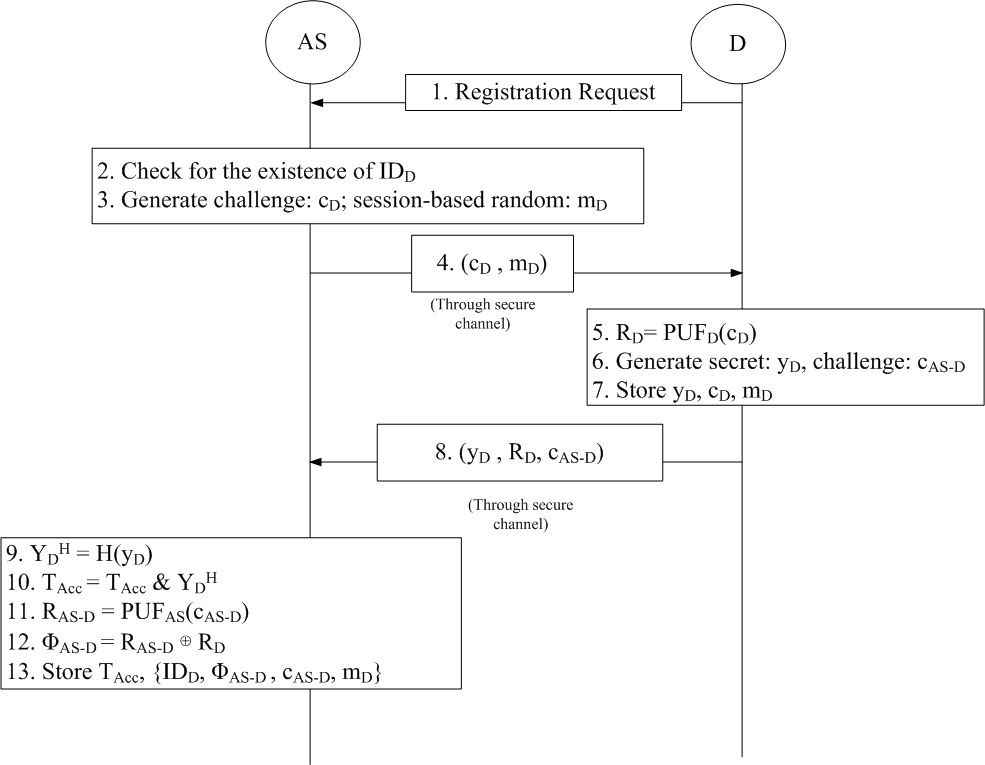
\includegraphics[width=0.82\textwidth]{EnrollmentPhase}
  \caption{Node Enrollment Phase of the base scheme (adapted from~\cite{das2026comsnets}).}
  \label{fig:base_enroll}
\end{figure}

\subsection{Node Authentication and Key Exchange Phase}

In the \textbf{Node Authentication Phase}, node $D$ authenticates itself to the AS
over an insecure public channel.
$D$ regenerates its PUF response $R_D = \mathsf{PUF}_D(c_D)$ and computes a mask
$H(R_D \| m_D \| ID_D \| ts_1)$, where $m_D$ is the current session-based random
obtained during enrollment.
The hashed witness $Y_D^H = H(y_D)$ is XORed with this mask and transmitted to the
AS along with the real device identity $ID_D$ and timestamp $ts_1$.

Upon receiving the message, AS reconstructs $R_D$ using $\Phi_D \oplus R_{AS\text{-}D}$,
regenerates the mask, unmasks $Y_D^{H'}$, and verifies authenticity by checking
$T_{\mathsf{Acc}}\ \&\ Y_D^{H'} = T_{\mathsf{Acc}}$.
If equality holds, the AS confirms that $D$ was previously registered.
Figure~\ref{fig:base_auth} shows the authentication phase.

\begin{figure}[!ht]
  \centering
  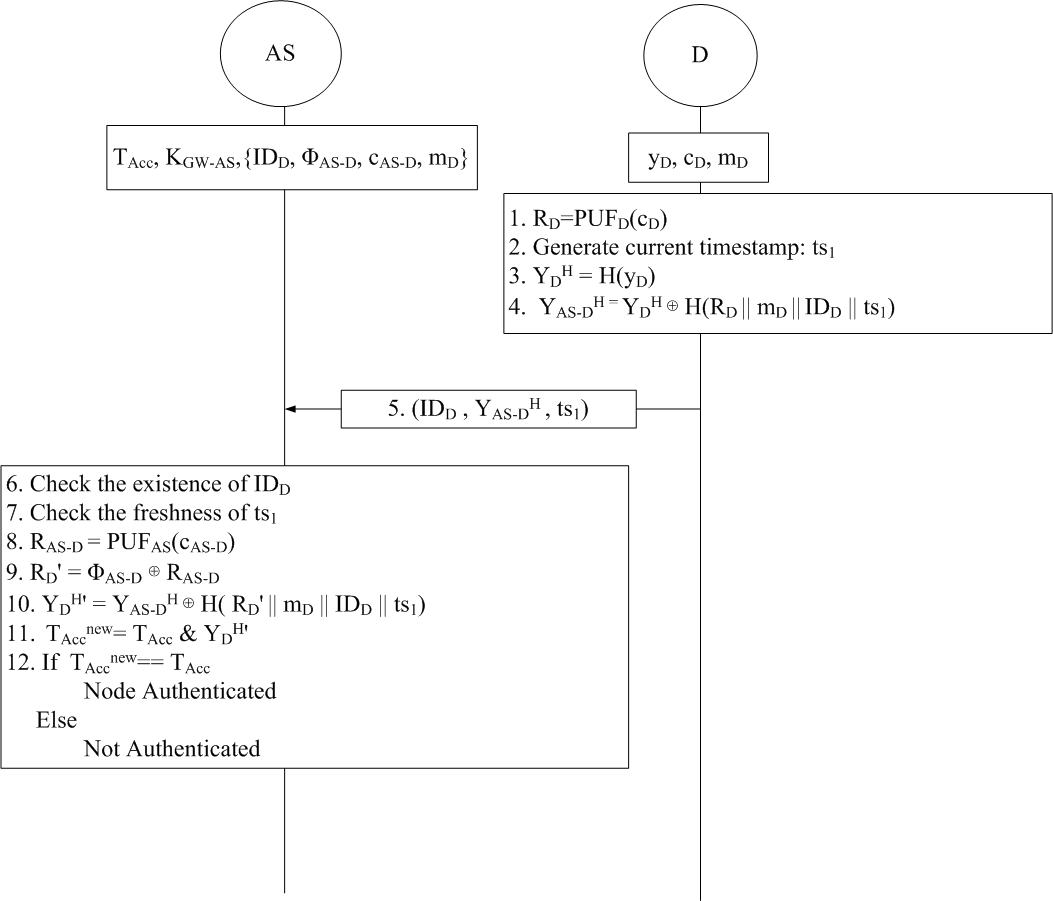
\includegraphics[width=0.82\textwidth]{AuthenticationPhase}
  \caption{Node Authentication Phase of the base scheme (adapted from~\cite{das2026comsnets}).}
  \label{fig:base_auth}
\end{figure}

The AS then generates a new session-based random $m_{\mathrm{new}} = H(n_1)$, where
$n_1$ is freshly chosen, replacing $m_D$ for the next session and providing forward
secrecy.
The session key for secure communication between the gateway and the node is computed
as $K_{GW\text{-}D} = H(R_D \| m_{\mathrm{new}})$.
AS constructs an authentication token containing $ID_D$, $ID_{AS}$, timestamp
$ts_{\mathrm{auth}}$, and the session key $K_{GW\text{-}D}$, encrypted under
$K_{GW\text{-}AS}$, and sends it to the gateway.
Figure~\ref{fig:base_keyex} illustrates this key exchange.

\begin{figure}[!ht]
  \centering
  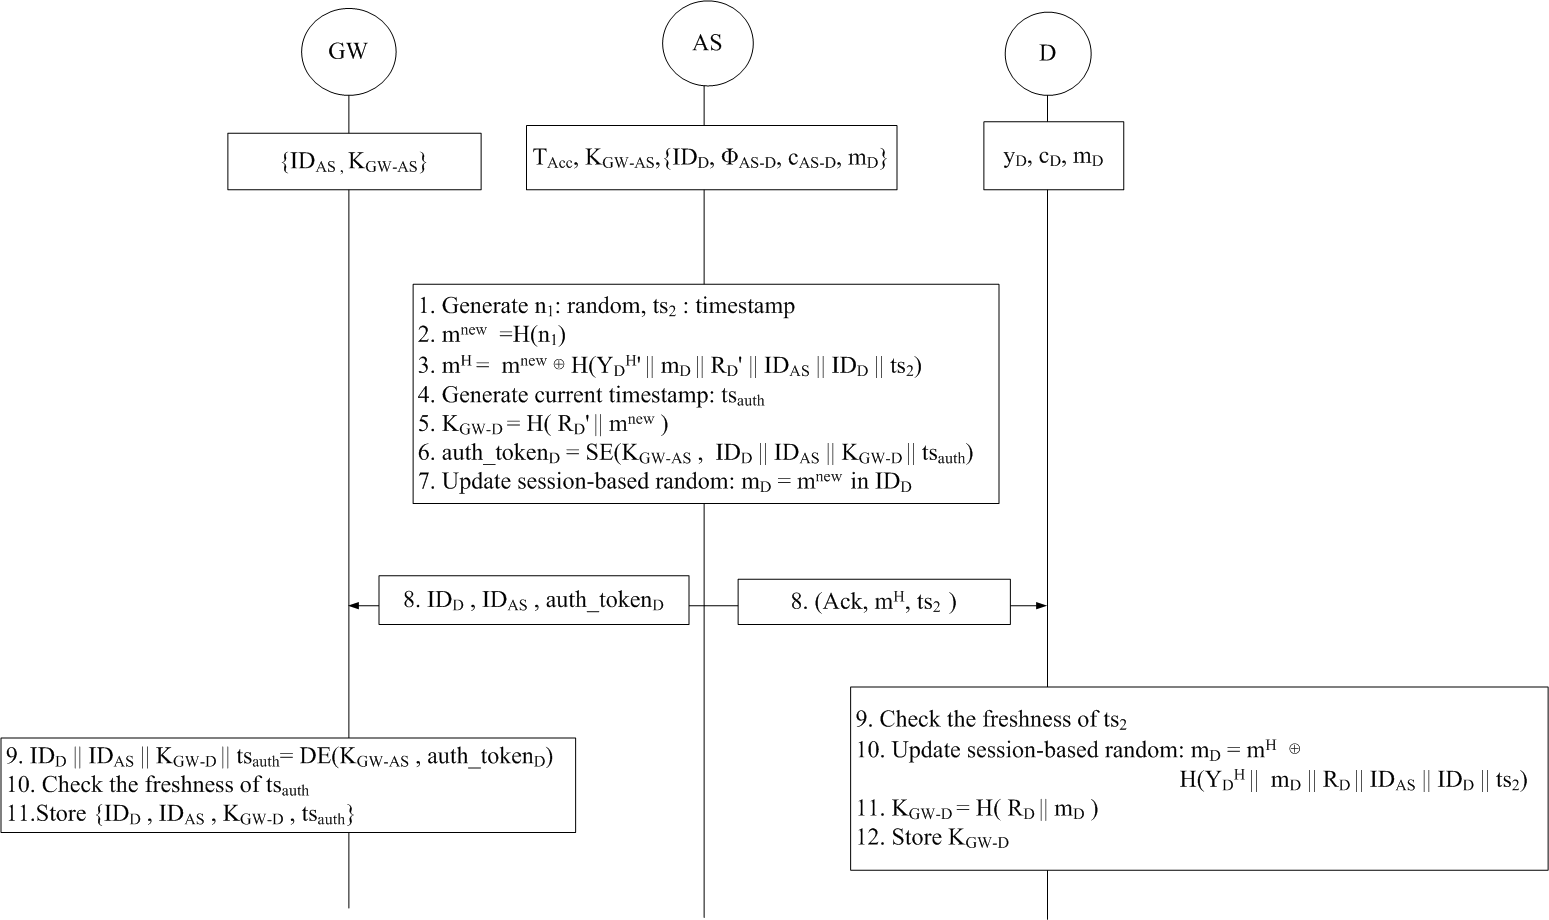
\includegraphics[width=0.95\textwidth]{KeyExchange}
  \caption{Node Key Exchange Phase of the base scheme (adapted from~\cite{das2026comsnets}).}
  \label{fig:base_keyex}
\end{figure}

\subsection{Privacy Gap in the Base Scheme}

Although the base scheme achieves decoupled and distributed authentication,
PUF-based security, lightweight computation, low storage overhead, and dynamic key
updates, it leaves two critical gaps unaddressed.

\textbf{Gap 1 — Identity Exposure:}
The real device identity $ID_D$ is transmitted in plaintext on the open channel in
every authentication session.
Since IoT networks usually operate in open and sometimes hostile environments, a
passive attacker who is just listening to the traffic can easily capture these
identity messages.
Even if other fields in the packet are protected, sending $ID_D$ in plain text is
enough for an attacker to link different authentication attempts from the same device.
Over time, this can allow long-term tracking, behaviour profiling, learning the
network structure, or even targeting a particular node for jamming.
In a multihop network, the problem becomes even worse because these packets move
across many intermediate nodes.

\textbf{Gap 2 — Desynchronisation:}
The base scheme stores only a single session nonce $m_D$ at the AS.
If the key-exchange response carrying the new $m_{\mathrm{new}}$ to device $D$ is
lost, $D$ retains the old $m_D$ while the AS has already advanced to $m_{\mathrm{new}}$.
On the next authentication attempt, $D$ constructs its authentication message using
the stale $m_D$, but the AS uses $m_{\mathrm{new}}$ to verify — the masks no longer
match, authentication fails, and the device must undergo costly full re-enrolment.

These gaps create the need for an improved authentication method that hides real
device identities, avoids linking across sessions, and adds anonymity without
breaking the lightweight and distributed design of the original scheme.

% ============================================================
%  CHAPTER 5 — Proposed Authentication Scheme
% ============================================================
\chapter{Proposed Authentication Scheme}
\label{ch:proposed}

\section{System Model and Assumptions}

The proposed scheme is designed to help nodes establish secure multihop
communications with the gateway.
To establish a secure communication, nodes should be authenticated by a trusted
authentication server.
A set of existing IoT nodes inside the network is entrusted with the responsibility
of authentication by the gateway in a distributed manner.
The gateway also shares a secret key with each of those responsible IoT
nodes/authentication servers.
The authentication server can be a parent or a non-parent node, which may be
\emph{decoupled}, preventing newly joined child nodes from overwhelming their parent
with biased authentication load.

IoT nodes are assumed to be embedded with a PUF and are capable of performing
various cryptographic operations, such as encryption/decryption, XOR, hashing,
bitwise AND, and concatenation.

Nodes $D$ and $AS$ are assumed to be the newly joined node and its authentication
server, respectively.
$GW$ represents the gateway symbolically.
$AS$ may be located at a single-hop or multi-hop distance from $D$.
It is assumed that $GW$ has already selected the authentication server set and has
established a shared secret key with each member of the set.
Let $\mathcal{AS}' = \{AS_1, AS_2, \ldots, AS_n\}$ be the set of authentication
servers selected by $GW$, such that $AS \in \mathcal{AS}'$.
$GW$ has a shared secret key $K_{GW\text{-}AS}$ with $AS$.
It is also assumed that $D$, whose distinct identifier is $ID_D$, possesses the
address of its authentication server $AS$ along with its unique identity $ID_{AS}$.
Table~\ref{tab:notations} elaborates symbols and functions incorporated in the
following scheme.

\begin{table}[!ht]
  \centering
  \caption{Notation Summary.}
  \label{tab:notations}
  \small
  \setlength{\tabcolsep}{8pt}
  \begin{tabular}{ll}
    \toprule
    Symbol & Description \\
    \midrule
    $D$, $AS$ & Newly joined device and its authentication server \\
    $GW$ & Gateway / root node \\
    $H(\cdot)$ & Collision-resistant hash function (SHA-256) \\
    $\mathsf{SE}(\cdot)$, $\mathsf{SD}(\cdot)$ & Symmetric encryption/decryption (AES-128) \\
    $\oplus$ & Bitwise XOR operation \\
    $\mathbin{\&}$ & Bitwise AND operation \\
    $c_D$, $c_{AS\text{-}D}$ & PUF challenges for $D$ (issued by $AS$) and $AS$ (by $D$) \\
    $m_D$ & Session-based random issued by $AS$ during enrolment \\
    $m_{\mathrm{curr}}$, $m_{\mathrm{old}}$ & Current and previous session-based randoms at $D$ and $AS$ \\
    $y_D$, $R_D$ & Unique secret and PUF response of $D$ \\
    $Y_D^H$ & Hashed unique secret: $H(y_D)$ \\
    $T_\mathsf{Acc}$ & Accumulated authentication value at $AS$ \\
    $\Phi_{AS\text{-}D}$ & PUF-response binding: $\mathsf{PUF}_{AS}(c_{AS\text{-}D}) \oplus R_D$ \\
    $\mathit{PID}_{\mathrm{curr}}$, $\mathit{PID}_{\mathrm{old}}$ & Current and previous pseudonyms of $D$ \\
    $K_{GW\text{-}D}$ & Session key between $GW$ and $D$ \\
    $K_{GW\text{-}AS}$ & Long-term shared key between $GW$ and $AS$ \\
    $ts_1$, $ts_2$, $ts_{\mathrm{auth}}$ & Timestamps for freshness verification \\
    \bottomrule
  \end{tabular}
\end{table}

There are mainly three phases: node enrolment, node authentication, and node session
key exchange.
The following sections elaborate on these phases.

\section{Node Enrolment Phase}

The node enrolment phase is the first phase undergone by a newly joined node $D$
with its authentication server $AS$.
Before entering this phase, it is assumed that $D$ has the required information
regarding $AS$: the address and unique identity ($ID_{AS}$) of $AS$.
$AS$ can lie at a single-hop or multi-hop distance from $D$.
This phase is assumed to be executed in a secure environment by establishing an
end-to-end encrypted channel between $D$ and $AS$.
Every newly joined node executes this phase once until it disconnects from the
network.
Figure~\ref{fig:prop_enroll} outlines the methodology of this phase.

\begin{figure}[!ht]
  \centering
  
\includegraphics[width=0.9\textwidth]{fig_enrollment}
  \caption{Proposed Scheme: Node Enrolment Phase with pseudonym initialisation.}
  \label{fig:prop_enroll}
\end{figure}

$D$ initiates the phase by sending a registration request along with its unique
identity $ID_D$ to $AS$ over the secure channel.
As a response, $AS$ generates a challenge $c_D$ from the predefined challenge set
$\mathbb{C}_D$ and a session-based random $m_D$; these are then forwarded securely
to $D$.
With $c_D$ as input to its embedded $\mathsf{PUF}_D$, $D$ obtains a unique response
$R_D = \mathsf{PUF}_D(c_D)$.
After this, $D$ generates its own unique secret value $y_D$, also a random number;
the security of the entire scheme critically depends on maintaining the
confidentiality of $y_D$.
$D$ also picks a reverse challenge $c_{AS\text{-}D}$ from the predefined challenge
set $\mathbb{C}_{AS\text{-}D}$ and sends $(y_D, R_D, c_{AS\text{-}D})$ back to
$AS$ through the secure channel.
$D$ then stores $\{y_D, c_D, m_D\}$.
Unlike~\cite{das2026comsnets}, which stores $m_D$ as a plain session random, the
proposed scheme retains it as the initial \emph{current} session random
$m_{\mathrm{curr}}$, seeding the pseudonym mechanism.

$AS$ inputs the secret $y_D$ to the hash function $H(\cdot)$, generating tag
$Y_D^H = H(y_D)$, and updates the accumulator as
$T_\mathsf{Acc} = T_\mathsf{Acc}\ \&\ Y_D^H$.
Further, $AS$ generates
$R_{AS\text{-}D} = \mathsf{PUF}_{AS}(c_{AS\text{-}D})$ and calculates
$\Phi_{AS\text{-}D} = R_{AS\text{-}D} \oplus R_D$.

\textbf{Pseudonym Initialisation (new in proposed scheme):}
The proposed scheme extends this base enrolment with pseudonym and dual-state
initialisation to eliminate $ID_D$ from all future open-channel messages.
Since $ID_D$ is transmitted only over this secure enrolment channel and must never
appear on the open channel again, $D$ will henceforth be identified by the rotating
pseudonym $\mathit{PID} = H(ID_D \| m_{\mathrm{curr}})$ in all future
authentication messages.
Because $H$ is one-way and $m_{\mathrm{curr}}$ is a private session random,
successive pseudonyms are computationally unlinkable by a channel observer.
$AS$ pre-computes $\mathit{PID}_{\mathrm{curr}} = H(ID_D \| m_{\mathrm{curr}})$
and sets $\mathit{PID}_{\mathrm{old}} = \perp$, $m_{\mathrm{old}} = \perp$,
forming the initial \emph{dual state}.
$AS$ therefore stores
$\{T_\mathsf{Acc}, ID_D, \Phi_{AS\text{-}D}, c_{AS\text{-}D}, m_{\mathrm{curr}},
m_{\mathrm{old}}, \mathit{PID}_{\mathrm{curr}}, \mathit{PID}_{\mathrm{old}}\}$.

\section{Node Authentication Phase}

The node authentication phase is the second phase of the proposed scheme.
Its main purpose is to authenticate $D$'s unique secret $y_D$ with $AS$.
Since this phase is executed over an open channel, $y_D$ must be communicated in
secure form, preventing it from being intercepted by adversaries.
This security is established through PUF-based challenge-response, producing a
secret key $R_D$, and the session-based random $m_{\mathrm{curr}}$, incorporating
unpredictability.
Both $R_D$ and $m_{\mathrm{curr}}$ are known only to $D$ and $AS$.
Figure~\ref{fig:prop_auth} illustrates the phase.

\begin{figure}[!ht]
  \centering
  
\includegraphics[width=0.9\textwidth]{fig_auth.png}
  \caption{Proposed Scheme: Node Authentication Phase with dual-state pseudonym lookup.}
  \label{fig:prop_auth}
\end{figure}

The phase is initiated by $D$.
$D$ regenerates $R_D = \mathsf{PUF}_D(c_D)$ from the stored challenge $c_D$
obtained during enrolment.
$D$ then computes its current pseudonym $\mathit{PID} = H(ID_D \| m_{\mathrm{curr}})$,
which is used in place of the real identity $ID_D$ in the outgoing message.
$D$ produces the hashed secret $Y_D^H = H(y_D)$ in XORed form as:
\begin{equation}
  Y_{AS\text{-}D}^H = H(y_D) \oplus H(R_D \| m_{\mathrm{curr}} \| \mathit{PID} \| ts_1).
\end{equation}
The XOR mask is the hash of $R_D$, the session-based random $m_{\mathrm{curr}}$,
the pseudonym $\mathit{PID}$, and the current timestamp $ts_1$.
The timestamp is used to provide replay protection to the XORed value
$Y_{AS\text{-}D}^H$.
The complete message $(\mathit{PID}, Y_{AS\text{-}D}^H, ts_1)$ is then sent to $AS$.

After receiving the message, $AS$ checks for the existence of an entry matching the
received $\mathit{PID}$.
In a departure from~\cite{das2026comsnets}, $AS$ performs a \textbf{dual-state
lookup}: it checks whether the received $\mathit{PID}$ matches
$\mathit{PID}_{\mathrm{curr}}$ or $\mathit{PID}_{\mathrm{old}}$ in its records.
A match on $\mathit{PID}_{\mathrm{old}}$ indicates that $D$ missed the Key Exchange
Phase delivery in the previous session and still holds the prior $m_{\mathrm{curr}}$;
in this case, $AS$ uses the stored $m_{\mathrm{old}}$ for the subsequent
verification, recovering from the desynchronisation without requiring re-enrolment.
$AS$ verifies the freshness of $ts_1$, reconstructs $R_D'$ as
$\Phi_{AS\text{-}D} \oplus \mathsf{PUF}_{AS}(c_{AS\text{-}D})$, regenerates the
same XOR mask, unmasks $Y_D^{H'}$, and then performs the bitwise AND check:
\begin{equation}
  T_\mathsf{Acc}^{\mathsf{new}} = T_\mathsf{Acc}\ \&\ Y_D^{H'}
  \stackrel{?}{=} T_\mathsf{Acc}.
\end{equation}
If $T_\mathsf{Acc}^{\mathsf{new}} = T_\mathsf{Acc}$, it proves that the unique
secret of $D$ is already a legitimate member of $AS$.
With the successful operation, the authentication of $D$ is completed by $AS$, and
$AS$ proceeds to the Key Exchange Phase.

\section{Node Session Key Exchange Phase}

This phase is executed by $AS$ to inform $GW$ about the authentication of the newly
joined node $D$ at the end of the authentication phase.
$AS$ uses an $\mathsf{auth\_token}_D$ to deliver the session key $K_{GW\text{-}D}$
to $GW$, facilitating session key generation between $GW$ and $D$.
The proposed scheme extends~\cite{das2026comsnets} by additionally deriving a fresh
pseudonym $\mathit{PID}_{\mathrm{new}} = H(ID_D \| m_{\mathrm{new}})$ at the end of
each session and carrying it within $\mathsf{auth\_token}_D$, so that $GW$ can
update its pseudonym mapping for $D$ and successive sessions remain unlinkable.
Figure~\ref{fig:prop_keyex} shows the phase.

\begin{figure}[!ht]
  \centering
  
\includegraphics[width=0.98\textwidth]{fig_keyex}
  \caption{Proposed Scheme: Node Session Key Exchange Phase with pseudonym rotation.}
  \label{fig:prop_keyex}
\end{figure}

$K_{GW\text{-}D}$ is calculated by $AS$ using the hashed output of $R_D'$ and
$m_{\mathrm{new}}$:
\begin{equation}
  K_{GW\text{-}D} = H(R_D' \| m_{\mathrm{new}}).
\end{equation}
$m_{\mathrm{new}}$ is computed by hashing a fresh random number $n_1$ generated by
$AS$ as $m_{\mathrm{new}} = H(n_1)$.
Further, $AS$ derives $\mathit{PID}_{\mathrm{new}} = H(ID_D \| m_{\mathrm{new}})$.
The session key $K_{GW\text{-}D}$, the identities $ID_{AS}$ and $ID_D$, the next
pseudonym $\mathit{PID}_{\mathrm{new}}$, and the authentication completion timestamp
$ts_{\mathrm{auth}}$ are encrypted under the shared key $K_{GW\text{-}AS}$ to form
$\mathsf{auth\_token}_D$.
$AS$ simultaneously sends $(m_H, ts_2)$ to $D$ and
$(\mathit{PID}_{\mathrm{new}}, ID_{AS}, \mathsf{auth\_token}_D)$ to $GW$, where
the masked session seed is:
\begin{equation}
  m_H = m_{\mathrm{new}} \oplus H(Y_D^{H'} \| m_{\mathrm{curr}} \| R_D' \|
  ID_{AS} \| \mathit{PID}_{\mathrm{curr}} \| ts_2).
\end{equation}
It then advances its records:
$m_{\mathrm{curr}} \leftarrow m_{\mathrm{new}}$,
$\mathit{PID}_{\mathrm{curr}} \leftarrow \mathit{PID}_{\mathrm{new}}$,
with $m_{\mathrm{old}}$ and $\mathit{PID}_{\mathrm{old}}$ retaining the superseded
values.

Obtaining $(m_H, ts_2)$, $D$ first verifies the freshness of $ts_2$, then recovers
$m_{\mathrm{new}}$ by regenerating the hash mask using its locally held
$Y_D^H$, $R_D$, $m_{\mathrm{curr}}$, $ID_{AS}$, $\mathit{PID}_{\mathrm{curr}}$, and
the received $ts_2$, and XORing with $m_H$.
$D$ establishes $K_{GW\text{-}D} = H(R_D \| m_{\mathrm{new}})$ and rotates its
pseudonym to $\mathit{PID}_{\mathrm{curr}} = H(ID_D \| m_{\mathrm{new}})$, thus
preparing itself for secure communication with $GW$.

$GW$ decrypts the token with $K_{GW\text{-}AS}$, verifies $ts_{\mathrm{auth}}$, and
extracts $K_{GW\text{-}D}$ and $\mathit{PID}_{\mathrm{new}}$.
$GW$ saves $\mathit{PID}_{\mathrm{curr}}$ as the previous pseudonym, sets
$\mathit{PID}_{\mathrm{new}}$ as the current one, and stores the session key against
both.

\section{Desynchronisation Recovery}

During the Key Exchange Phase, $AS$ simultaneously dispatches two packets: one to
$GW$ carrying $(\mathit{PID}_{\mathrm{new}}, ID_{AS}, \mathsf{auth\_token}_D)$,
and one to $D$ carrying $(m_H, ts_2)$.
Loss of either packet leads to a different desynchronisation scenario, each handled
without re-enrolment.

If the $AS \to D$ packet $(m_H, ts_2)$ is lost, $D$ retains its stale
$m_{\mathrm{curr}}$, so the pseudonym it computes in the next session equals
$\mathit{PID}_{\mathrm{old}}$ from $AS$'s perspective.
$AS$ recognises this via the dual-state lookup and resumes from the consistent prior
state, restoring synchronisation without any re-enrolment overhead.

Algorithm~\ref{alg:desync} shows how the scheme adapts the Authentication and Key
Exchange Phases to recover without re-enrolment.

\begin{algorithm}[!ht]
\caption{Desynchronisation Recovery}
\label{alg:desync}
\begin{algorithmic}[1]
\Statex \textbf{Precondition:} $D$ holds stale $m_{\mathrm{curr}} = m_{\mathrm{old}}$;\;
       $AS$ holds $(m_{\mathrm{curr}},\,m_{\mathrm{old}},\,
       \mathit{PID}_{\mathrm{curr}},\,\mathit{PID}_{\mathrm{old}})$
\Statex
\Statex \textit{Authentication Phase}
\State $\mathit{PID} \gets H(\mathit{ID}_D \| m_{\mathrm{curr}})$
       \hfill\Comment{stale $m_{\mathrm{curr}}$ $\Rightarrow$ $\mathit{PID} = \mathit{PID}_{\mathrm{old}}$}
\State $D \to AS$: $(\mathit{PID},\; Y_{AS\text{-}D}^H,\; ts_1)$
\If{$\mathit{PID} = \mathit{PID}_{\mathrm{curr}}$}
    \State $AS$ verifies using $m_{\mathrm{curr}}$ \hfill\Comment{normal path}
\ElsIf{$\mathit{PID} = \mathit{PID}_{\mathrm{old}}$}
    \State $AS$ verifies using $m_{\mathrm{old}}$ \hfill\Comment{desync detected}
\Else
    \State $AS$ rejects $D$
\EndIf
\Statex
\Statex \textit{Key Exchange Phase (desync path)}
\State $n_1 \gets \mathsf{rand}()$
\State $m_{\mathrm{new}} \gets H(n_1)$
\State $m_H \gets m_{\mathrm{new}} \oplus
       H\!\left(Y_D^{H'} \| m_{\mathrm{old}} \| R_D' \|
       \mathit{ID}_{AS} \| \mathit{PID}_{\mathrm{old}} \| ts_2\right)$
\State $AS \to D$: $(m_H,\; ts_2)$
\State $m_{\mathrm{new}} \gets m_H \oplus
       H\!\left(Y_D^{H} \| m_{\mathrm{curr}} \| R_D \|
       \mathit{ID}_{AS} \| \mathit{PID} \| ts_2\right)$
       \hfill\Comment{$D$ uses own $m_{\mathrm{curr}} = m_{\mathrm{old}}$}
\State $m_{\mathrm{old}} \gets m_{\mathrm{curr}}$;\quad
       $m_{\mathrm{curr}} \gets m_{\mathrm{new}}$;\quad
       $\mathit{PID} \gets H(\mathit{ID}_D \| m_{\mathrm{curr}})$
\Statex \textbf{Result:} $D$ and $AS$ re-synchronised; $\mathit{PID}$ rotated
\end{algorithmic}
\end{algorithm}

The dual-state mechanism tolerates a single consecutive Key Exchange Phase loss.
Two or more consecutive losses exhaust both slots, requiring re-enrolment — a
deliberate trade-off between storage overhead and recovery depth.

% ============================================================
%  CHAPTER 6 — Security Analysis
% ============================================================
\chapter{Security Analysis}

\section{Formal Security Analysis}

The proposed scheme is translated into ProVerif~\cite{blanchet2018proverif} queries
under the Dolev--Yao adversary model~\cite{dolev1983security}, where the adversary
has full control of the public channel and can intercept, replay, modify, and inject
messages.
All 19 queries are verified and all are satisfied.
Figure~\ref{fig:proverif} shows the verification summary.

\begin{figure}[!ht]
  \centering
  
\includegraphics[width=0.98\textwidth]{fig_proverif}
  \caption{ProVerif verification output — all 19 queries satisfied.}
  \label{fig:proverif}
\end{figure}

\subsection{Protocol Correspondence (Q1--Q9)}

Nine correspondence queries verify that the protocol steps happen in the correct
order and that no adversary can skip or forge a step.

\textbf{Q1--Q2 (Enrolment correspondence):}
Q1 (injective) and Q2 (non-injective) check enrolment integrity: a device can
only be registered at the authentication server after it has explicitly initiated the
enrolment process.
This rules out any possibility of a device being enrolled without its own
participation.

\textbf{Q3--Q6 (Two-round authentication correspondence):}
These four queries check both directions of both authentication rounds.
The device side (Q3, Q5) verifies that the device receives the server's
acknowledgement and the fresh timestamp $ts_2$ only after it first sent a valid
authentication request, preventing replay of a stale acknowledgement.
The server side (Q4, Q6) verifies that the authentication server completes its
processing only after receiving a structurally correct request from the device.

\textbf{Q7 (Cross-round binding):}
Q7 binds the Authentication and Key Exchange phases: the PUF response $R_D$ and
the session seed $m_{\mathrm{curr}}$ that the device commits during authentication
are proven to be exactly the same values used in the key exchange.
This rules out an active adversary who might try to substitute credentials between
phases.

\textbf{Q8--Q9 (Token delivery and data communication correspondence):}
These queries cover key exchange and data communication: the device recovers the new
session seed $m_{\mathrm{new}}$ only after it legitimately sent the key-exchange
request, and data communication is established only after successful key exchange.

\subsection{Secrecy and Forward Secrecy (Q10--Q14)}

\textbf{Q10--Q12 (Session key secrecy):}
Three queries verify the secrecy of the session key
$K_{GW\text{-}D} = H(R_D \| m_{\mathrm{new}})$ from three views: device, AS, and
gateway.
Even though the adversary observes all traffic on the public channel, it cannot
reconstruct $K_{GW\text{-}D}$ because the PUF response $R_D$ is never transmitted
and $m_{\mathrm{new}}$ is always delivered XOR-masked.

\textbf{Q13 (Forward secrecy of $m_{\mathrm{new}}$):}
A separate query confirms forward secrecy: the rotated session seed $m_{\mathrm{new}}$
itself remains secret.
Even if an adversary somehow recovers a current session key, it gains nothing about
future sessions, because each $m_{\mathrm{new}}$ is derived from an independently
generated fresh nonce.

\textbf{Q14 ($R_D$ secrecy):}
The PUF response $R_D$ is never transmitted; this query confirms it cannot be derived
from the observed channel traffic.

\subsection{Anonymity Preservation (Q15)}

\textbf{Q15 ($ID_D$ anonymity):}
The most significant secrecy result concerns the real device identity $ID_D$.
After enrolment, $ID_D$ is never sent over the open channel again.
Every subsequent message instead carries the pseudonym
$\mathit{PID} = H(ID_D \| m_{\mathrm{curr}})$.
ProVerif formally confirms that no attacker, even one who intercepts and manipulates
every single message on the network, can recover $ID_D$ from the observed traffic.

This result supports device anonymity.
However, anonymity is only meaningful if the pseudonym used in one session cannot be
linked to the pseudonym used in the next.
The forward-secrecy query (Q13) addresses this: because $m_{\mathrm{new}}$ is proven
secret, consecutive pseudonyms $H(ID_D \| m_{\mathrm{curr}})$ and
$H(ID_D \| m_{\mathrm{new}})$ are computationally indistinguishable to any
observer, making it difficult for an adversary who collects pseudonyms from multiple
sessions to determine whether they belong to the same physical device.

\subsection{Timestamp Secrecy and Offline Guessing Resistance (Q16--Q19)}

\textbf{Q16 ($ts_2$ secrecy):}
The session timestamp $ts_2$ is embedded in the XOR mask protecting $m_{\mathrm{new}}$.
This query confirms that $ts_2$ is not derivable from the public transcript without
knowing the other mask components.

\textbf{Q17--Q19 (Weak secrecy / offline guessing resistance):}
These weak-secrecy queries confirm that the session key $K_{GW\text{-}D}$, the
session seed $m_{\mathrm{new}}$, and the hashed witness $Y_D^H$ cannot be guessed
from the public transcript even by an adversary with unlimited offline dictionary
power.
This closes the gap against brute-force and dictionary attacks that target the key
directly from captured packets.

\section{Informal Analysis}

\subsection{Replay Attack Resistance}

The Enrolment Phase is executed over a secure channel and is immune to replay.
The Authentication and Key Exchange Phases embed timestamps ($ts_1$, $ts_2$,
$ts_{\mathrm{auth}}$) and the session-based random $m_{\mathrm{curr}}$ into the hash
masks.
A replayed message with a stale timestamp or stale $m_{\mathrm{curr}}$ will fail the
freshness check at $AS$, $D$, or $GW$ respectively.

\subsection{MITM Attack Resistance}

The Enrolment Phase is conducted over an encrypted channel, which precludes MITM.
In the Authentication and Key Exchange Phases, the PUF response $R_D$
(device-specific, unreproducible) and session random $m_{\mathrm{curr}}$ (private to
$D$ and $AS$) are embedded in every XOR mask.
Without $R_D$ and the current $m_{\mathrm{curr}}$, no adversary can forge a valid
masked tag $Y_{AS\text{-}D}^H$ or unmask $m_H$.

\subsection{Device Anonymity}

$ID_D$ is transmitted only once, over the secure enrolment channel, and is never
exposed on the open network again.
All open-channel messages use $\mathit{PID} = H(ID_D \| m_{\mathrm{curr}})$,
which is refreshed to $H(ID_D \| m_{\mathrm{new}})$ after every key exchange.
Because $m_{\mathrm{new}}$ is derived from a freshly generated nonce $n_1$,
successive pseudonyms are computationally unlinkable.

\subsection{Desynchronisation Recovery}

Packet loss can occur at three distinct points in the Authentication and Key Exchange
Phases, each handled without requiring re-enrolment.

If the acknowledgement and fresh timestamp $ts_2$ sent by $AS$ to $D$ at the end of
the authentication phase are lost in transit, $D$ does not advance its internal state.
Since $AS$ has not yet performed any state update at this stage, both entities remain
consistent.
Upon timeout, $D$ retransmits the authentication request with the same $\mathit{PID}$
and $ts_1$, and the exchange proceeds normally.

The primary desynchronisation scenario arises when the Key Exchange Phase response
$(m_H, ts_2)$ is lost.
In this case, $AS$ has already advanced its state to $m_{\mathrm{new}}$ and rotated
the pseudonym to $\mathit{PID}_{\mathrm{new}}$, while $D$ retains the previous
$m_{\mathrm{curr}}$.
On the subsequent authentication attempt, $D$ constructs its pseudonym from the
stale $m_{\mathrm{curr}}$, producing $\mathit{PID}_{\mathrm{old}}$.
$AS$ recognises this via the dual-state lookup and resumes from the consistent prior
state.

If the token forwarded from $AS$ to $GW$ is lost, $D$ re-initiates from the
Authentication Phase; the dual-state storage at $AS$ ensures that this
re-authentication succeeds and a fresh token is forwarded to $GW$.

\subsection{Forward Secrecy}

$K_{GW\text{-}D} = H(R_D \| m_{\mathrm{new}})$.
Compromise of a session key does not reveal previous session keys because
$m_{\mathrm{new}}$ is independently generated from a fresh nonce and $R_D$ is
PUF-derived.

% ============================================================
%  CHAPTER 7 — Performance Analysis
% ============================================================
\chapter{Performance Analysis}

\section{Theoretical Performance Analysis}

\subsection{Computational Cost}

The computational cost is a crucial deterministic factor ensuring the security and
efficiency of an authentication scheme.
The Python cryptographic library \texttt{pycrypto} is used in a Windows environment
to measure the computational cost of core cryptographic functions, such as SHA-256
($T_{\mathsf{hash}}$), AES Encryption/Decryption ($T_{\mathsf{aes}}$), and random
generation ($T_{\mathsf{rand}}$).
The PUF operation cost ($T_{\mathsf{puf}}$) is taken from prior benchmarks on the
same platform~\cite{zheng2022puf}.
Benchmark averages over 100 iterations are: $T_{\mathsf{rand}} = 0.0018$\,ms,
$T_{\mathsf{puf}} = 0.0522$\,ms, $T_{\mathsf{hash}} = 0.0353$\,ms,
$T_{\mathsf{aes}} = 0.0867$\,ms.

\subsubsection{Enrolment Phase}

To execute the node enrolment phase:
\begin{itemize}
  \item $AS$ computes two random generations ($T_{\mathsf{rand}}$), one PUF
    operation ($T_{\mathsf{puf}}$), and two hash operations ($T_{\mathsf{hash}}$)
    for pseudonym initialisation.
  \item $D$ executes two random generations ($T_{\mathsf{rand}}$) and one PUF
    operation ($T_{\mathsf{puf}}$).
\end{itemize}

Hence, the total computational cost per node enrolment amounts to
$2T_{\mathsf{puf}} + 2T_{\mathsf{hash}} + 4T_{\mathsf{rand}} = \mathbf{0.18}$\,ms.
Table~\ref{tab:comp_enroll} compares the enrolment computational cost.

\begin{table}[!ht]
  \centering
  \caption{Computational Cost Comparison: Enrolment Phase.}
  \label{tab:comp_enroll}
  \small
  \setlength{\tabcolsep}{5pt}
  \begin{tabular}{lll}
    \toprule
    Scheme & Operations & Cost (ms) \\
    \midrule
    LAAKA~\cite{ali2024laaka}          & $3T_\mathsf{hash}$ & 0.11 \\
    Zhou~\cite{zhou2024auth}           & $T_\mathsf{puf}+2T_\mathsf{hash}+3T_\mathsf{rand}$ & 0.13 \\
    Zheng et al.~\cite{zheng2022puf}   & $2T_\mathsf{puf}+8T_\mathsf{hash}+4T_\mathsf{aes}+5T_\mathsf{rand}$ & 0.69 \\
    He et al.~\cite{he2023lightweight} & $4T_\mathsf{hash}+T_\mathsf{aes}+T_\mathsf{rand}$ & 0.23 \\
    \textbf{Proposed}                  & $2T_\mathsf{puf}+2T_\mathsf{hash}+4T_\mathsf{rand}$ & \textbf{0.18} \\
    \bottomrule
  \end{tabular}
\end{table}

\subsubsection{Authentication and Key Exchange Phase}

In the proposed scheme, $D$ and $AS$ both execute one PUF operation
($T_{\mathsf{puf}}$).
\begin{itemize}
  \item $D$ additionally performs six hash operations ($T_{\mathsf{hash}}$):
    pseudonym computation, unique secret hash, and XOR mask in the Authentication
    Phase, followed by mask recovery, session key derivation, and pseudonym
    rotation in the Key Exchange Phase.
  \item $AS$ performs five hash operations ($T_{\mathsf{hash}}$), along with one
    AES encryption ($T_{\mathsf{aes}}$) for the gateway token and one random
    generation ($T_{\mathsf{rand}}$) for $m_{\mathrm{new}}$.
  \item $GW$ runs one AES decryption ($T_{\mathsf{aes}}$) to recover the session
    key and updated pseudonym from the forwarded token.
\end{itemize}

This leads to a total cost of
$2T_{\mathsf{puf}} + 11T_{\mathsf{hash}} + 2T_{\mathsf{aes}} + T_{\mathsf{rand}}
= \mathbf{0.67}$\,ms.
Table~\ref{tab:comp_auth} compares the authentication and key exchange computational
cost.

\begin{table}[!ht]
  \centering
  \caption{Computational Cost Comparison: Authentication \& Key Exchange Phase.}
  \label{tab:comp_auth}
  \small
  \setlength{\tabcolsep}{5pt}
  \begin{tabular}{lll}
    \toprule
    Scheme & Operations & Cost (ms) \\
    \midrule
    LAAKA~\cite{ali2024laaka}          & $16T_\mathsf{hash}$ & 0.56 \\
    Zhou~\cite{zhou2024auth}           & $15T_\mathsf{hash}$ & 0.53 \\
    Zheng et al.~\cite{zheng2022puf}   & $2T_\mathsf{puf}+6T_\mathsf{hash}+4T_\mathsf{aes}+5T_\mathsf{rand}$ & 0.67 \\
    He et al.~\cite{he2023lightweight} & $11T_\mathsf{hash}+5T_\mathsf{aes}+2T_\mathsf{ecc}$ & 1.74 \\
    \textbf{Proposed}                  & $2T_\mathsf{puf}+11T_\mathsf{hash}+2T_\mathsf{aes}+T_\mathsf{rand}$ & \textbf{0.67} \\
    \bottomrule
  \end{tabular}\\[4pt]
  \small$T_\mathsf{ecc}=0.461$\,ms (scaled from He et al.~\cite{he2023lightweight} hardware ratios).
\end{table}

\subsection{Communication Cost}

Communication cost is a core feature for analysing the performance of an
authentication scheme, based on the number of message exchanges and their sizes (in
bits).
It is assumed that identities and timestamps are 32\,bits, along with nonces, hashes,
challenges, responses, and ciphertexts as 256\,bits, ensuring a fair comparison.

\subsubsection{Enrolment Phase}

During the node enrolment phase, $D$ enrols itself with $AS$, executing three message
exchanges: (1)~$ID_D$ (32\,b) from $D$ to $AS$; (2)~$c_D$ (256\,b) and $m_D$
(256\,b) from $AS$ to $D$; (3)~$y_D$ (256\,b), $R_D$ (256\,b), and $c_{AS\text{-}D}$
(256\,b) from $D$ to $AS$.
Total enrolment communication cost: \textbf{1312\,bits}.
Table~\ref{tab:comm_enroll} shows the comparison.

\begin{table}[!ht]
  \centering
  \caption{Communication Cost Comparison: Enrolment Phase.}
  \label{tab:comm_enroll}
  \small
  \setlength{\tabcolsep}{6pt}
  \begin{tabular}{lcc}
    \toprule
    Scheme & \# Messages & Cost (bits) \\
    \midrule
    LAAKA~\cite{ali2024laaka}          & 3 & 2592 \\
    Zhou~\cite{zhou2024auth}           & 5 & 1344 \\
    Zheng et al.~\cite{zheng2022puf}   & 3 & 1600 \\
    He et al.~\cite{he2023lightweight} & 2 & 1280 \\
    \textbf{Proposed}                  & 3 & \textbf{1312} \\
    \bottomrule
  \end{tabular}
\end{table}

\subsubsection{Authentication and Key Exchange Phase}

The authentication and key exchange phase is executed using three message
communications.
Message 1 ($D \to AS$): $\mathit{PID}$ (256\,b) + $Y_{AS\text{-}D}^H$ (256\,b) +
$ts_1$ (32\,b).
Message 2 ($AS \to D$): $m_H$ (256\,b) + $ts_2$ (32\,b).
Message 3 ($AS \to GW$): $\mathit{PID}_{\mathrm{new}}$ (256\,b) + $ID_{AS}$ (32\,b)
+ $\mathsf{auth\_token}_D$ (256\,b).
Total: \textbf{1376\,bits}.
Table~\ref{tab:comm_auth} shows the comparison.

\begin{table}[!ht]
  \centering
  \caption{Communication Cost Comparison: Authentication \& Key Exchange Phase.}
  \label{tab:comm_auth}
  \small
  \setlength{\tabcolsep}{6pt}
  \begin{tabular}{lcc}
    \toprule
    Scheme & \# Messages & Cost (bits) \\
    \midrule
    LAAKA~\cite{ali2024laaka}          & 3 & 2400 \\
    Zhou~\cite{zhou2024auth}           & 4 & 2464 \\
    Zheng et al.~\cite{zheng2022puf}   & 3 & 1600 \\
    He et al.~\cite{he2023lightweight} & 3 & 1120 \\
    \textbf{Proposed}                  & 3 & \textbf{1376} \\
    \bottomrule
  \end{tabular}
\end{table}

Das~\cite{das2026comsnets} requires 928\,bits; the 448-bit increase in the proposed
scheme directly reflects the widening of the device identifier from a 32-bit $ID_D$
to a 256-bit pseudonym $\mathit{PID}$ — the direct cost of adding device anonymity
to all open-channel communications.

\FloatBarrier
\section{Simulation-Based Performance Analysis}
\label{sec:sim}

A simulation-based performance evaluation has been conducted using the COOJA
simulator within the Contiki-NG framework.
Three complementary studies are reported.
\begin{enumerate}
  \item \textbf{Overall per-device comparison:} Proposed scheme vs.\
    LAAKA~\cite{ali2024laaka} and Zhou~\cite{zhou2024auth} in a fixed 100-node
    network (1 GW, 79 AS nodes with 2 active, 20 newly joined devices).
  \item \textbf{AS pool-size study:} Active AS nodes varied from 2 to 10.
  \item \textbf{Network scalability study:} Total node count varied across
    $N \in \{30, 50, 80, 100\}$.
\end{enumerate}
All results are averaged over five independent random seeds.
Table~\ref{tab:simparams} lists the common simulation parameters.

\begin{table}[!ht]
  \centering
  \caption{Simulation Parameters.}
  \label{tab:simparams}
  \small
  \setlength{\tabcolsep}{5pt}
  \begin{tabular}{ll}
    \toprule
    Parameter & Value \\
    \midrule
    Simulator            & COOJA (Contiki-NG) \\
    Mote type            & Emulated IoT nodes \\
    Topology (study i)   & 100 nodes: 1 GW, 79 AS (2 active), 20 devices \\
    Routing protocol     & RPL Lite \\
    MAC/PHY              & CSMA / IEEE 802.15.4 \\
    Phases measured      & Enrolment, Authentication, Key Exchange \\
    Schemes compared     & Proposed, LAAKA~\cite{ali2024laaka}, Zhou~\cite{zhou2024auth} \\
    Active AS (study ii) & 2, 5, 10 \\
    Network size (study iii) & $N \in \{30, 50, 80, 100\}$ \\
    Random seeds         & 5 per configuration \\
    \bottomrule
  \end{tabular}
\end{table}

\subsection{Overall Per-Device Cost}

For 20 newly joined nodes in a fixed 100-node network, the proposed scheme
demonstrated a consistent advantage over LAAKA and Zhou.
As shown in Figure~\ref{fig:sim_total}(a), the proposed scheme achieves a reduction
of \textbf{42.8\,\%} and \textbf{34.6\,\%} in total per-device energy consumption
over LAAKA and Zhou, respectively.
Similarly, a reduction of \textbf{42.7\,\%} and \textbf{35.3\,\%} is demonstrated
in total per-device CPU time (Figure~\ref{fig:sim_total}(b)).
The dominant savings arise in the authentication and key exchange phase, where the
proposed scheme consumes 28.87\,mJ against 77.97\,mJ for LAAKA and 57.06\,mJ for
Zhou.
Due to the incorporation of fewer message exchanges and computationally lightweight
hash-XOR operations, the proposed scheme has minimised radio activity and
computational load compared to the message-intensive and cryptographically heavier
LAAKA and Zhou schemes.

\begin{figure}[!ht]
  \centering
  
\includegraphics[width=0.92\textwidth]{fig_sim_total}
  \caption{Per-device mean total cost, all phases:
           (a)~energy and (b)~CPU time, 100-node network, 10 seeds.}
  \label{fig:sim_total}
\end{figure}

\subsection{Authentication Server Pool Size}

In the decoupled design, the gateway selects any capable node as the authentication
server, so the size of the AS pool directly influences load distribution and overall
network performance.
The performance of the proposed scheme, LAAKA, and Zhou is evaluated by varying the
number of active AS nodes from 2 to 10.

Considering the total energy consumption (Figure~\ref{fig:sim_as}(a)), a reduction
of approximately \textbf{42\,\%} is demonstrated by the proposed scheme over LAAKA
at every AS count.
Both schemes improve from AS = 2 to AS = 10, with the proposed scheme dropping from
1065\,mJ to 936\,mJ and LAAKA from 1827\,mJ to 1631\,mJ, suggesting that a pool of
10 AS nodes is near-optimal for a 20-device network.
As shown in Figure~\ref{fig:sim_as}(b), a reduction of approximately 42\,\% in
total CPU time is demonstrated over LAAKA across all AS counts.
Zhou's total cost remains flat at approximately 1503\,mJ in energy and 24.4\,s in
CPU time regardless of AS pool size, confirming that its gateway-coupled design is
insensitive to AS selection diversity.

\begin{figure}[!ht]
  \centering
  \begin{subfigure}[b]{0.72\linewidth}
    
\includegraphics[width=\linewidth]{fig_sim_as_energy}
    \caption{Total energy vs.\ number of active AS nodes.}
  \end{subfigure}
  \par\vspace{8pt}
  \begin{subfigure}[b]{0.72\linewidth}
    
\includegraphics[width=\linewidth]{fig_sim_as_cpu}
    \caption{Total CPU time vs.\ number of active AS nodes.}
  \end{subfigure}
  \caption{Authentication cost vs.\ AS pool size (20 devices, 5 seeds).}
  \label{fig:sim_as}
\end{figure}

\subsection{Network Scalability}

The performance of authentication schemes is also analysed by considering their
scalability with respect to total network size $N$, varied from 30 to 100 nodes.
Considering the total energy consumption (Figure~\ref{fig:sim_network}(a)), a
reduction of \textbf{42.2\,\%} and \textbf{50.6\,\%} is demonstrated by the
proposed scheme at $N = 100$ over LAAKA (898\,mJ) and Zhou (1051\,mJ), respectively.
Similarly, as shown in Figure~\ref{fig:sim_network}(b), a reduction of 42.5\,\% and
50.6\,\% is demonstrated with respect to total CPU time over LAAKA (14.6\,s) and
Zhou (17.0\,s), respectively.
LAAKA and Zhou exhibit steeper energy and CPU growth with increasing $N$ because
their heavier per-device cryptographic load accumulates faster as the device count
grows.

\begin{figure}[!ht]
  \centering
  \begin{subfigure}[b]{0.72\linewidth}
    
\includegraphics[width=\linewidth]{fig_sim_net_energy}
    \caption{Total energy vs.\ network size $N$.}
  \end{subfigure}
  \par\vspace{8pt}
  \begin{subfigure}[b]{0.72\linewidth}
    
\includegraphics[width=\linewidth]{fig_sim_net_cpu}
    \caption{Total CPU time vs.\ network size $N$.}
  \end{subfigure}
  \caption{Network scalability: total energy and CPU time vs.\ $N$.}
  \label{fig:sim_network}
\end{figure}

\subsection{Desynchronisation Recovery}
\label{sec:desync_perf}

During the Key Exchange Phase, the AS simultaneously dispatches two packets: one to
the gateway carrying $(\mathit{PID}_{\mathrm{new}}, ID_{AS},
\mathsf{auth\_token}_D)$, and one to the device carrying $(m_H, ts_2)$.
Desynchronisation arises when the packet destined for the device is lost in transit.

Das~\cite{das2026comsnets} stores only a single nonce state at the AS.
When the device re-authenticates using the old $m_{\mathrm{curr}}$, the AS has no
means to recognise it and rejects the request.
The device must therefore undergo a full re-enrolment before a new authentication
and key exchange can succeed.
The proposed scheme eliminates this penalty through its dual-state mechanism.

Figure~\ref{fig:desync_bar} presents a per-device energy and CPU time comparison
of a single authentication round under two conditions: normal operation (before any
packet loss) and recovery (the round immediately following a desynchronisation
event), evaluated over a 100-node multi-hop RPL network, 20 devices, and 5 seeds.
As shown in Figure~\ref{fig:desync_bar}(a), Das~\cite{das2026comsnets} incurs
134.8\,mJ per recovery round, a 118.3\,\% increase over its normal round cost of
61.8\,mJ, reflecting the overhead of a failed authentication attempt followed by
full re-enrolment.
The proposed scheme's recovery round costs 87.2\,mJ, statistically indistinguishable
from its normal round (98.6\,mJ), confirming that the dual-state mechanism incurs
zero additional overhead during recovery.
Compared directly, the proposed scheme reduces per-device recovery energy by
\textbf{47.6\,mJ (35.3\,\%)} over Das~\cite{das2026comsnets}.
The CPU time results in Figure~\ref{fig:desync_bar}(b) exhibit the same pattern:
Das~\cite{das2026comsnets} incurs 2.185\,s per recovery round against 1.413\,s for
the proposed scheme, yielding a \textbf{35.3\,\% reduction} in execution time.

\begin{figure}[!ht]
  \centering
  
\includegraphics[width=0.95\textwidth]{fig_desync_bar}
  \caption{Per-device desynchronisation recovery cost: (a)~energy and
           (b)~CPU time for a normal round vs.\ a recovery round, averaged over
           20 devices and 5 seeds in a 100-node RPL network.}
  \label{fig:desync_bar}
\end{figure}

\FloatBarrier
\section{Hardware-Based Performance Analysis}

Hardware-based performance analysis plays a crucial role as it validates the
feasibility of the proposed authentication scheme by implementing it on physical IoT
devices, incorporating real hardware environment conditions.

The proposed scheme and the baseline authentication schemes
LAAKA~\cite{ali2024laaka} and Zhou~\cite{zhou2024auth} are implemented on a
\textbf{Raspberry Pi~4B} platform, equipped with a quad-core 64-bit ARM Cortex-A72
processor operating at 1.5\,GHz.
A uniform hardware setup is maintained across all compared authentication schemes,
ensuring a fair and consistent comparison of energy consumption and CPU time.
The implementation considers two Raspberry Pi~4B platforms as IoT nodes: one
performing the role of the newly joined device, and the other functioning as the
authentication server.
A Linux-based laptop is leveraged as the gateway.
Each of the three entities maintains direct TCP communication with the others.
Energy consumption is estimated using the active power profile of the Raspberry
Pi~4B (3.8\,W) multiplied by the measured wall-clock time per authentication round.

As illustrated in Figure~\ref{fig:hw_comparison}(a), the proposed scheme achieves
the lowest energy consumption of \textbf{0.286\,J} per authentication round,
reducing energy by \textbf{52.5\,\%} and \textbf{14.2\,\%} compared to LAAKA
(0.602\,J) and Zhou (0.333\,J), respectively.
The CPU time results, as shown in Figure~\ref{fig:hw_comparison}(b), further confirm
this efficiency: the proposed scheme achieves \textbf{0.0753\,s} per round, reducing
CPU time by \textbf{52.5\,\%} and \textbf{14.1\,\%} over LAAKA (0.1585\,s) and
Zhou (0.0877\,s), respectively.
These reductions are consistent with the lightweight XOR-hash operations and
decoupled AS design of the proposed scheme, which translate directly to measurable
gains in physical energy and execution time on real hardware.

\begin{figure}[!ht]
  \centering
  
\includegraphics[width=0.95\textwidth]{fig_hw_comparison}
  \caption{Hardware-based performance: (a)~energy consumption and (b)~CPU time
           per authentication round on Raspberry Pi~4B
           (Proposed vs.\ LAAKA vs.\ Zhou).}
  \label{fig:hw_comparison}
\end{figure}

The inconsistency between hardware and simulation-based results arises due to the
disparity in scale, where a 100-node network is assumed in simulation whereas the
hardware setup involves only two Raspberry Pi platforms.

% ============================================================
%  CHAPTER 8 — Future Scope
% ============================================================
\chapter{Future Scope}

The proposed scheme addresses the primary gaps of identity exposure and
desynchronisation vulnerability in the base scheme, but several directions remain
open for future investigation.

\section{Reducing Authentication Server Storage Overhead}

The dual-state storage mechanism introduced in this work effectively prevents
desynchronisation by retaining both the current and previous session state
$(m_{\mathrm{curr}}, m_{\mathrm{old}}, \mathit{PID}_{\mathrm{curr}},
\mathit{PID}_{\mathrm{old}})$ at the Authentication Server.
While this eliminates the need for costly re-enrolment after a single
packet-loss event, it comes at the cost of doubling the per-device memory
footprint at the AS.
In low-power IoT networks where the AS is itself a resource-constrained node,
this additional storage can become a bottleneck as the number of registered
devices grows.

Future work should investigate lightweight strategies to bound this overhead.
One approach is time-bounded state expiry: the old state slot
$(\mathit{PID}_{\mathrm{old}}, m_{\mathrm{old}})$ is automatically invalidated
after a configurable timeout window, reclaiming storage without permanently
breaking authentication for well-behaved devices.
A complementary approach is policy-driven eviction, where the AS preferentially
retains old state only for devices known to operate in lossy environments
(e.g., at the edge of the network), while applying a single-state policy to
devices with historically reliable links.
Combining these with a compact probabilistic data structure (such as a Bloom
filter for fast PID lookup) could further reduce both memory and lookup latency
on severely constrained AS nodes.

\section{Anonymity of Authentication Servers}

In the current scheme, device identity is fully protected: the real $ID_D$ is
replaced by a rotating pseudonym $\mathit{PID}$ on all open-channel messages,
and no channel observer can link two sessions to the same physical device.
However, the identity of the Authentication Server ($ID_{AS}$) is still
transmitted in plaintext as part of the Key Exchange Phase message
$(\mathit{PID}_{\mathrm{new}}, ID_{AS}, \mathsf{auth\_token}_D)$ forwarded to
the gateway, and as part of the XOR mask components used by the device.

This partial transparency means that a passive adversary monitoring the channel
can identify which node is acting as the AS for a given authentication session,
infer the network topology, and potentially target the AS node for jamming or
impersonation.
In a fully anonymous system, the AS identity should be concealed from
eavesdroppers just as the device identity is.

Future work should extend the pseudonym mechanism to cover $ID_{AS}$ as well,
perhaps by having the gateway assign a rotating AS pseudonym
$\mathit{PID}_{AS} = H(ID_{AS} \| k_{AS})$ refreshed per session,
where $k_{AS}$ is a gateway-AS shared secret unknown to the channel.
Care must be taken to preserve the gateway's ability to route the authentication
token correctly and to update its AS-pseudonym mapping after each session,
mirroring the dual-state design already used for device pseudonyms.
Achieving complete end-to-end anonymity — where neither device nor AS identity
is recoverable from channel traffic — would close the remaining privacy gap and
make the scheme suitable for the most adversarial deployment environments.

% ============================================================
%  CHAPTER 9 — Conclusion
% ============================================================
\chapter{Conclusion}

This report presented the design, security analysis, and performance evaluation of a
lightweight, anonymous, and decoupled distributed authentication scheme for multihop
IoT networks.

Starting from the base scheme of Das~\cite{das2026comsnets}, two critical gaps were
identified: the exposure of the real device identity $ID_D$ on the public channel in
every authentication session, and the absence of desynchronisation recovery when a
key-exchange packet is lost in transit.
The proposed scheme addresses both gaps while preserving the core features of the
base scheme, including PUF-based secret derivation, hash-based accumulator
authentication, decoupled authentication server selection, and the lightweight
hash-XOR computational structure.

Device anonymity is preserved through \textbf{per-session pseudonym rotation}, where
a rotating pseudonym $\mathit{PID} = H(ID_D \| m_{\mathrm{curr}})$ replaces the
real device identity in all open-channel communications.
Because $m_{\mathrm{curr}}$ is refreshed from a fresh nonce after every successful
key exchange, consecutive pseudonyms are computationally unlinkable by any channel
observer.
A \textbf{dual-state mechanism} maintained at both the authentication server and the
gateway stores both the current and immediately prior session state, enabling seamless
recovery from a single packet-loss event without re-enrolment.

Formal verification in ProVerif confirms all 19 security queries under the Dolev--Yao
adversary model: authentication correspondence, session key secrecy, forward secrecy,
anonymity preservation ($ID_D$ secrecy), and offline guessing resistance.

COOJA/Contiki-NG simulations on 100-node RPL networks confirm practical suitability:
\begin{itemize}
  \item The proposed scheme achieves a per-device three-phase energy of 52.21\,mJ,
    reducing total energy by \textbf{42.8\,\%} over LAAKA and \textbf{34.6\,\%}
    over Zhou.
  \item Consistent gains are observed across varying network sizes
    ($N \in \{30, 50, 80, 100\}$) and AS pool sizes (2 to 10).
  \item Desynchronisation recovery reduces per-device recovery energy by
    \textbf{35.3\,\%} over the base scheme with zero additional overhead.
\end{itemize}

Hardware measurements on Raspberry Pi~4B confirm energy reductions of \textbf{52.5\,\%}
over LAAKA and \textbf{14.2\,\%} over Zhou per authentication round.

The proposed scheme is the first to simultaneously achieve decoupled distributed
authentication, PUF-based secret derivation, hash-based accumulator authentication,
authentication secret update, device anonymity via pseudonym, and desynchronisation
recovery — all at low computational and communication overhead suitable for
resource-constrained multihop IoT devices.

% ============================================================
%  BIBLIOGRAPHY
% ============================================================
\bibliographystyle{IEEEtran}
\bibliography{ref}

\end{document}
